% !Mode:: "TeX:UTF-8"

\begin{frame}{微分方程(Differential Equation)}
	\linespread{1.5}
	\begin{center}
		\resizebox{!}{6cm}{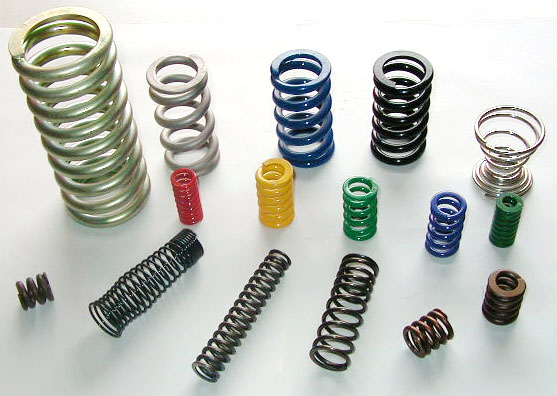
\includegraphics{./images/ch07/springs.jpg}}
	\end{center}
\end{frame}

\section{微分方程的概念}

\begin{frame}{预习概念}
	\linespread{1.5}
	\bf
	\begin{itemize}
	  \item 微分方程,常微分方程
	  \item 微分方程的解,通解,特解,初值问题
	  \item 隐式解,隐式通解,积分曲线
	  \item 可分离变量的方程
	  \item 齐次方程
	\end{itemize}
\end{frame}

\begin{frame}{思考}
	\linespread{1.2}
	\begin{enumerate}
	  \item 含有$n$个任意常数的解即为$n$阶线性微分方程的通解?\\
	  \onslide<2->{{\b 必须是相互独立的任意常数!}}
	  \item 微分方程通解就是其全部的解?\\
	  \onslide<3->{(\alert{$\times$}),{\b 例如:$y'=3\sin x\cos^2y$}}
	  \item 什么是微分方程“阶”和“次”?\\
	  \onslide<4->{{\b “阶”:导数的阶;“次”:幂次}}
	  \item 求解一阶微分方程的关键是什么?\\
	  \onslide<5->{{\b 变量分离,然后分别积分}}
	\end{enumerate}
\end{frame}

\begin{frame}{课后作业与预习要点}
	\linespread{1.2}
	
\end{frame}

\begin{frame}[<+->]{小结}
	\linespread{1.5}
	\begin{enumerate}
	  \item {\bf 微分方程的相关概念:}
	  \begin{itemize}
	    \item 解、通解、特解、初值问题
	  \end{itemize}
	  \item {\bf 一阶微分方程的解法}
	  \begin{itemize}
	    \item 可分离变量方程
	    \item 齐次方程
	    \item 一阶线性方程
	    \item Bernoulli方程
	  \end{itemize}
	\end{enumerate}
\end{frame}